\documentclass[11pt]{article}
\usepackage[utf8]{inputenc}
\usepackage{parskip}
\usepackage[a4paper, margin=1in]{geometry}
\usepackage{graphicx}
\usepackage{hyperref}
\usepackage{listings}
\usepackage{array}
\usepackage[capitalise,noabbrev]{cleveref}
\usepackage{rotating}

% Custom json syntax highlightning
\usepackage{bera}
\usepackage{xcolor}

\definecolor{background}{HTML}{EEEEEE}
 
\lstdefinestyle{mystyle}{
	basicstyle=\ttfamily\small,
	backgroundcolor=\color{background},
	breakatwhitespace=false,        
    frame=lines,   
    breaklines=true,                 
    captionpos=b,                    
    keepspaces=true,                 
    numbers=left,                    
    numbersep=5pt,                  
    showspaces=false,                
    showstringspaces=false,
    showtabs=false,                  
	tabsize=4,
	numbers=left,
	numberstyle=\tiny\color{black},
	numbersep=10pt,
	framexleftmargin=5pt,
	framexrightmargin=5pt,
}

\lstset{style=mystyle}

\definecolor{jsonstring}{RGB}{61,107,42}
\colorlet{jsonpunct}{red!60!black}
\definecolor{jsondelim}{RGB}{20,105,176}
\colorlet{jsonnumb}{magenta!60!black}

\lstdefinelanguage{json}{
	stringstyle={\color{jsonstring}},
	string = [d]{"},
    literate=
     *{0}{{{\color{jsonnumb}0}}}{1}
      {1}{{{\color{jsonnumb}1}}}{1}
      {2}{{{\color{jsonnumb}2}}}{1}
      {3}{{{\color{jsonnumb}3}}}{1}
      {4}{{{\color{jsonnumb}4}}}{1}
      {5}{{{\color{jsonnumb}5}}}{1}
      {6}{{{\color{jsonnumb}6}}}{1}
      {7}{{{\color{jsonnumb}7}}}{1}
      {8}{{{\color{jsonnumb}8}}}{1}
      {9}{{{\color{jsonnumb}9}}}{1}
      {:}{{{\color{jsonpunct}{:}}}}{1}
      {,}{{{\color{jsonpunct}{,}}}}{1}
      {\{}{{{\color{jsondelim}{\{}}}}{1}
      {\}}{{{\color{jsondelim}{\}}}}}{1}
      {[}{{{\color{jsondelim}{[}}}}{1}
      {]}{{{\color{jsondelim}{]}}}}{1},
}

\definecolor{javared}{rgb}{0.6,0,0} % for strings
\definecolor{javagreen}{rgb}{0.25,0.5,0.35} % comments
\definecolor{javapurple}{rgb}{0.5,0,0.35} % keywords
\definecolor{javadocblue}{rgb}{0.25,0.35,0.75} % javadoc
\definecolor{javablue}{HTML}{348B98}
 
\lstset{language=Java,
	keywordstyle=\color{javapurple}\bfseries,
	stringstyle=\color{javared},
	commentstyle=\color{javagreen},
	morecomment=[s][\color{javadocblue}]{/**}{*/},
	emph=[1]% Java Classes
    {%
		AggregateIterable,
		FindIterable,
        Document,
        Arrays,
        Aggregates,
        Accumulators,
        Bson,
        RuntimeException,
        User,
        Session,
        Movie,
        Adapter,
        Sorts,
        Projections,
    },
	emphstyle=[1]{\color{javablue}},
}

\renewcommand{\arraystretch}{1.5}

\title{Task 2 -- Movie Database\\ 
	\Large Final Report}
\date{\today}
\author{Federico Fregosi, Mirko Laruina,\\
        Riccardo Mancini, Gianmarco Petrelli}

\begin{document}
\pagenumbering{gobble}
\maketitle
\vfill
\setcounter{tocdepth}{2}
\tableofcontents
\vfill
\clearpage
\setcounter{page}{1}
\pagenumbering{arabic}

\section{Specifications}

\subsection{Application Overview}
The application is an aggregator of movies and movie ratings with the purpose 
of providing logged users statistics and informations about a large set of movies.
Logged-in user can also rate movies they have watched while not logged-in users 
may still use the service to browse movie rankings and statistics but they are not
able to give their rate. Only movies released in Italy are considered.

All users can search a movie and view its details (e.g., title, original title, duration, 
cast, ...) along with its average rating from users and from external sources. 

In addition, all users can browse the list of movies sorting and filtering it by many parameters
(e.g. year, genre, country, actors, ...).

System administrators can view all user profile pages and ban users. In order to do that, he can 
check the full history of ratings. Once a user is banned, he can no longer log in and his username and email cannot be used by new users.

The movie database will be built upon the publicly available IMDb dataset.

The ratings will be gathered also by periodically scraping external websites 
(e.g., Rotten Tomatoes, Coming Soon, MyMovies).

\subsection{Actors}
Anonymous user, registered user, administrator and updater ``bot''.

\subsection{Requirement Analysis}

\subsubsection{Functional Requirements}
An \textbf{anonymous user} must be able to register in order to become a 
\textit{registered user}. Login is carried out using username and password selected 
by the user when registering. Username must be unique. A valid email address is
also required in order to register. An email cannot be used more than once.

Both \textbf{anonymous user} and \textbf{registered user} must be able to:
\begin{itemize}
	\item view details and average rating of a specific movie
	\item view a list of movies and filter it by many parameters. Combined filters 
	are also allowed
	\item view aggregated statistics about movies: the user can choose on which field to aggregate movies (year, country, actor, director, genre) and additional filters (like the movie browsing feature). E.g. the user might want to see the ranking of the countries with the best movies in the last 10 years.
\end{itemize}

A \textbf{registered user} must be able to rate a movie, in addition to what anonymous
user can do. A registered user must also be able to manage his profile. In the profile a
registered user can:
\begin{itemize}
	\item check, add and modify his personal data
	\item browse the history of his rates
	\item view aggregated statistics about his profile (i.e. most viewed genre,
	most recurrent actor, etc...) based on his rated movies
	\item delete the account
\end{itemize}
Finally, a registered user can logout in any moment.

An \textbf{administrator} is a special registered user who must be able to ban users.
In order to do that, an administrator can check a global rating history to retrieve information
about all the application's activity, and to check every user's profile.
Banned user's rating are automatically removed from the database. Email and username
of banned users cannot be used again.

The \textbf{updater ``bot''} is not a real user but an entity used to periodically update the database in order to add new movies and update external ratings. 

\subsubsection{Non-Functional Requirements}
\begin{itemize}
	\item \textbf{Availability}: the Database must be replicated in order to be always available.
	Write operations on the Database can be eventually consistent.
	\item \textbf{Scalability}: the application must be able to scale to an arbitrary number of servers.
	\item \textbf{Security}: passwords must be stored in a secure way.
	\item \textbf{Responsive UI}: Client-side application must provide a responsive view both for pc, 
	laptops and mobile devices.
\end{itemize}

\section{Design}

\subsection{Use-case diagram}

\begin{sidewaysfigure}[h!]
    \centering
    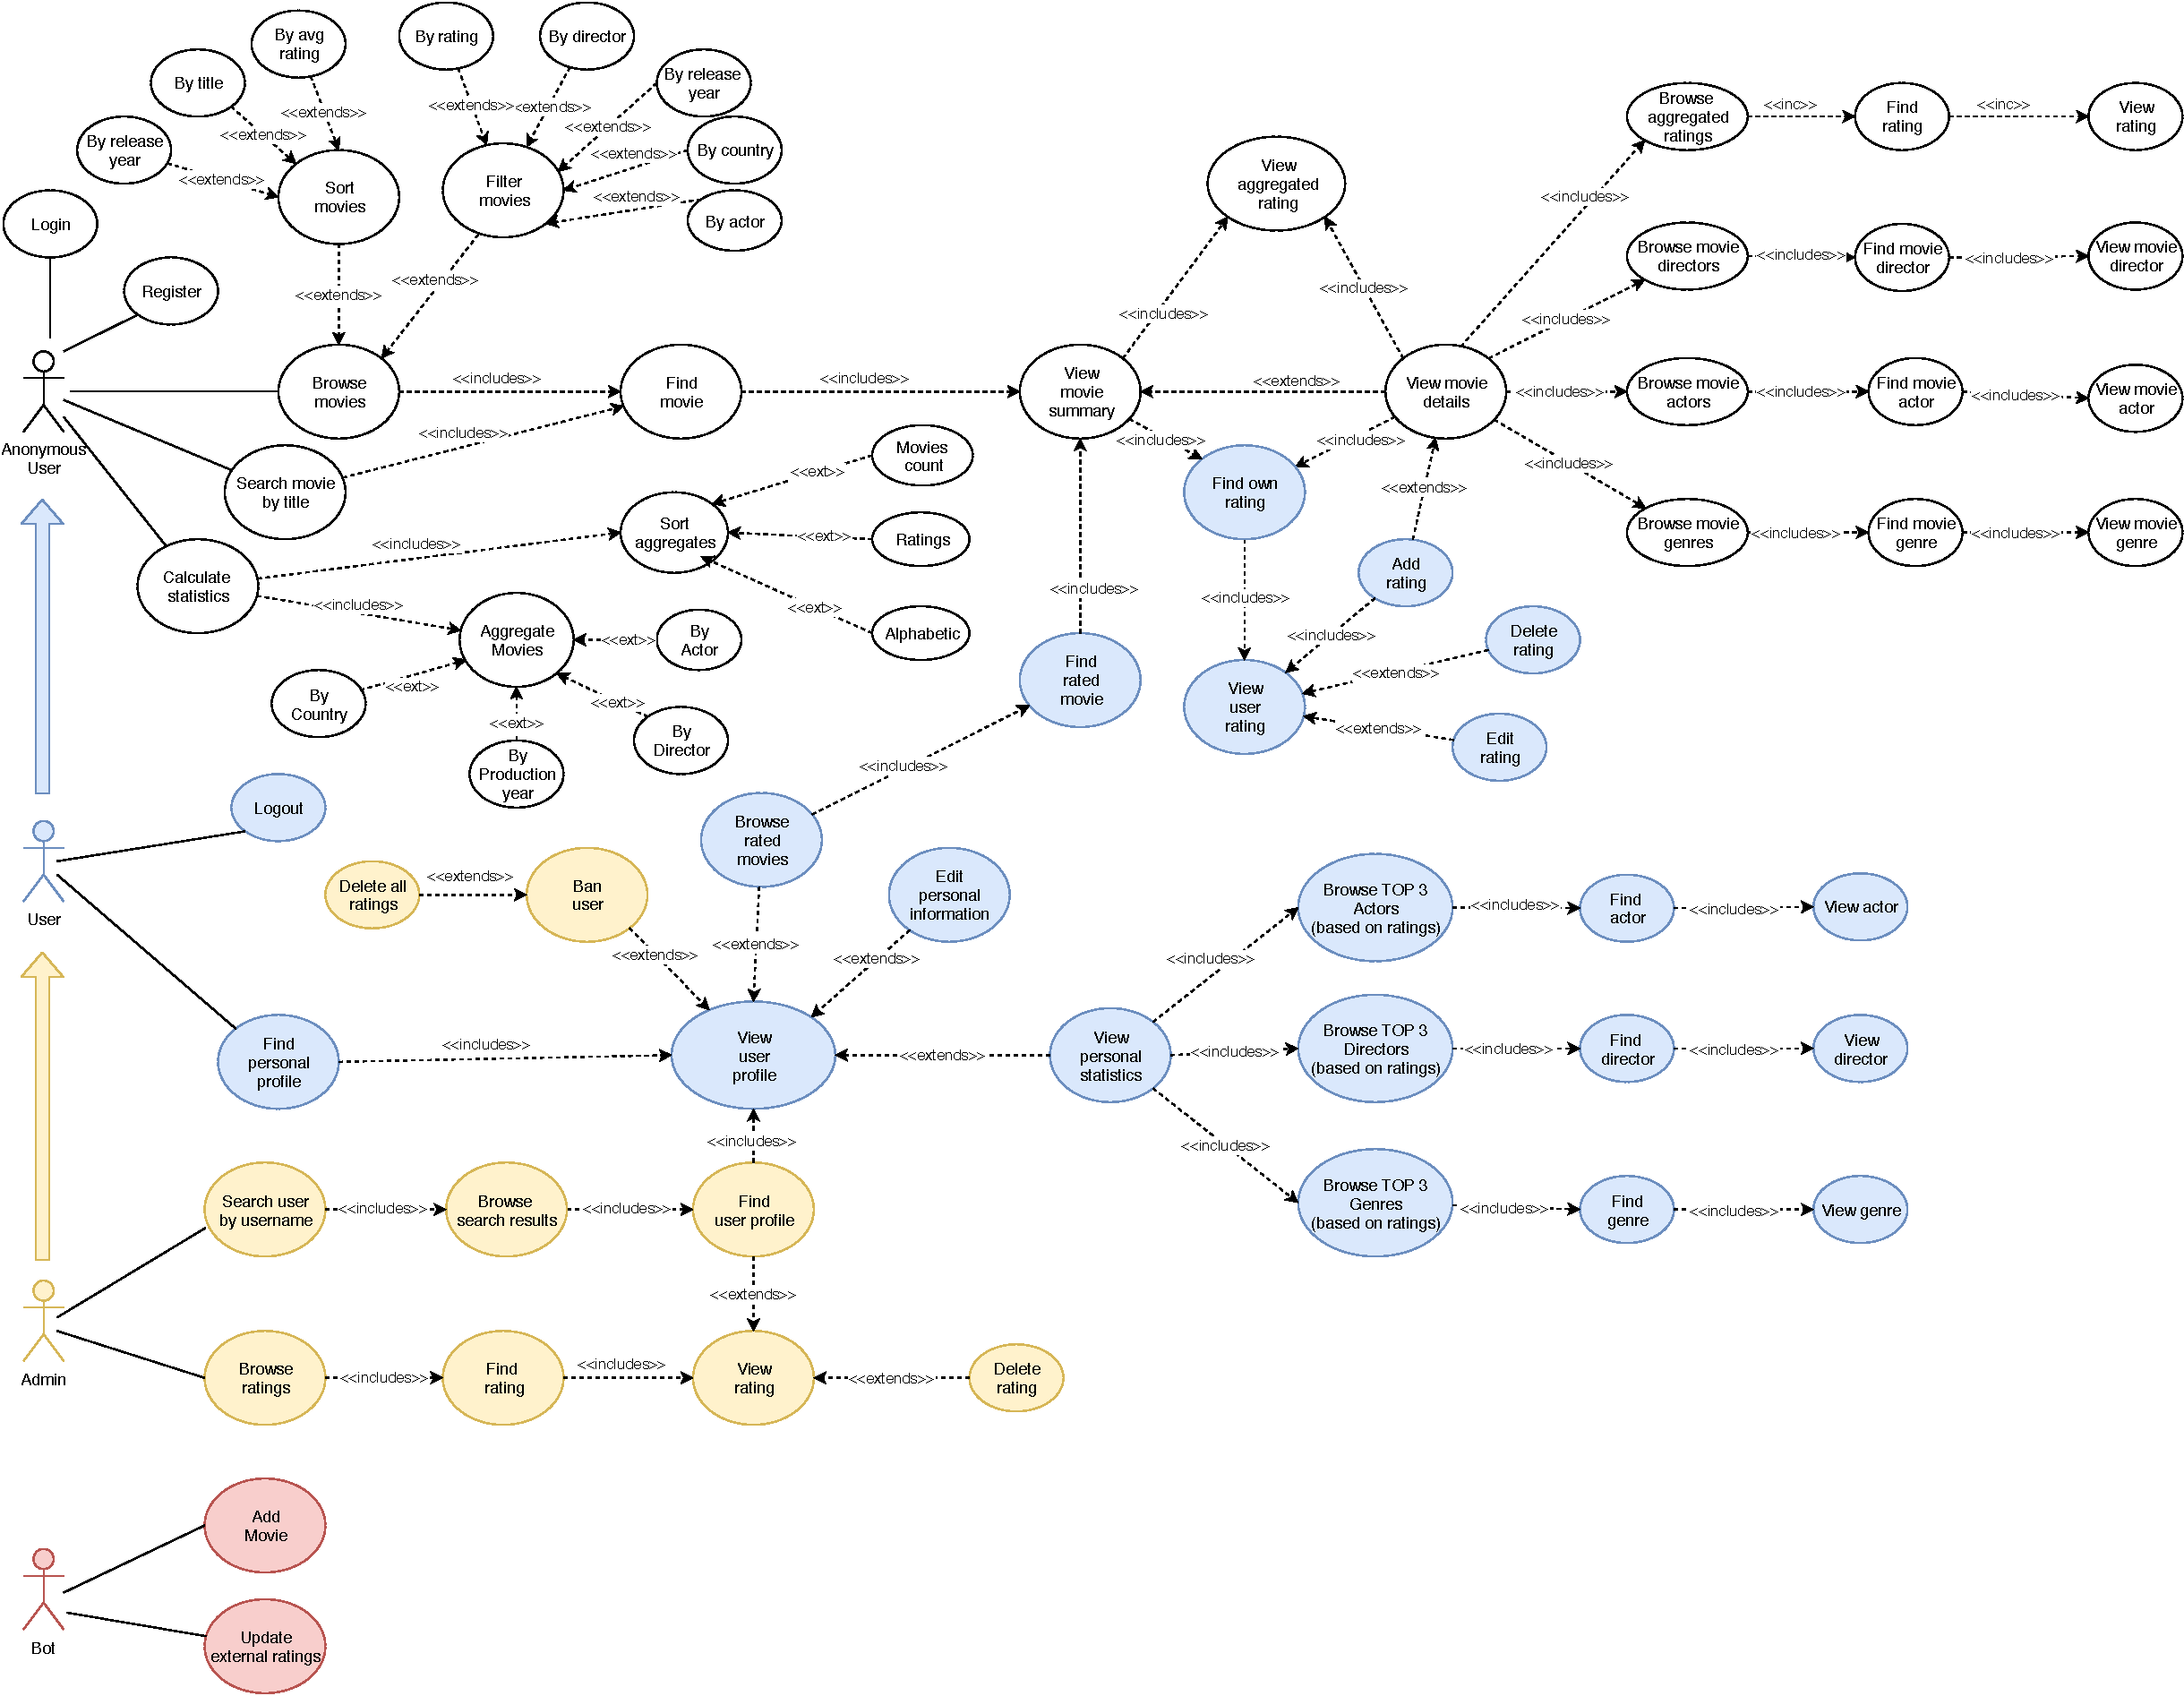
\includegraphics[height=18cm]{figs/use_case.pdf}
    \caption{Use-case diagram}
    \label{fig:usecase}
\end{sidewaysfigure}

The use-case diagram is shown in \cref{fig:usecase}. Different colors are used to highlight cases that are exclusive of some actors: white cases are referred to all users; blue cases are referred to registered user and admin; yellow cases are exclusive of the admin.

\subsection{Class diagram}

\begin{figure}[h!]
    \centering
    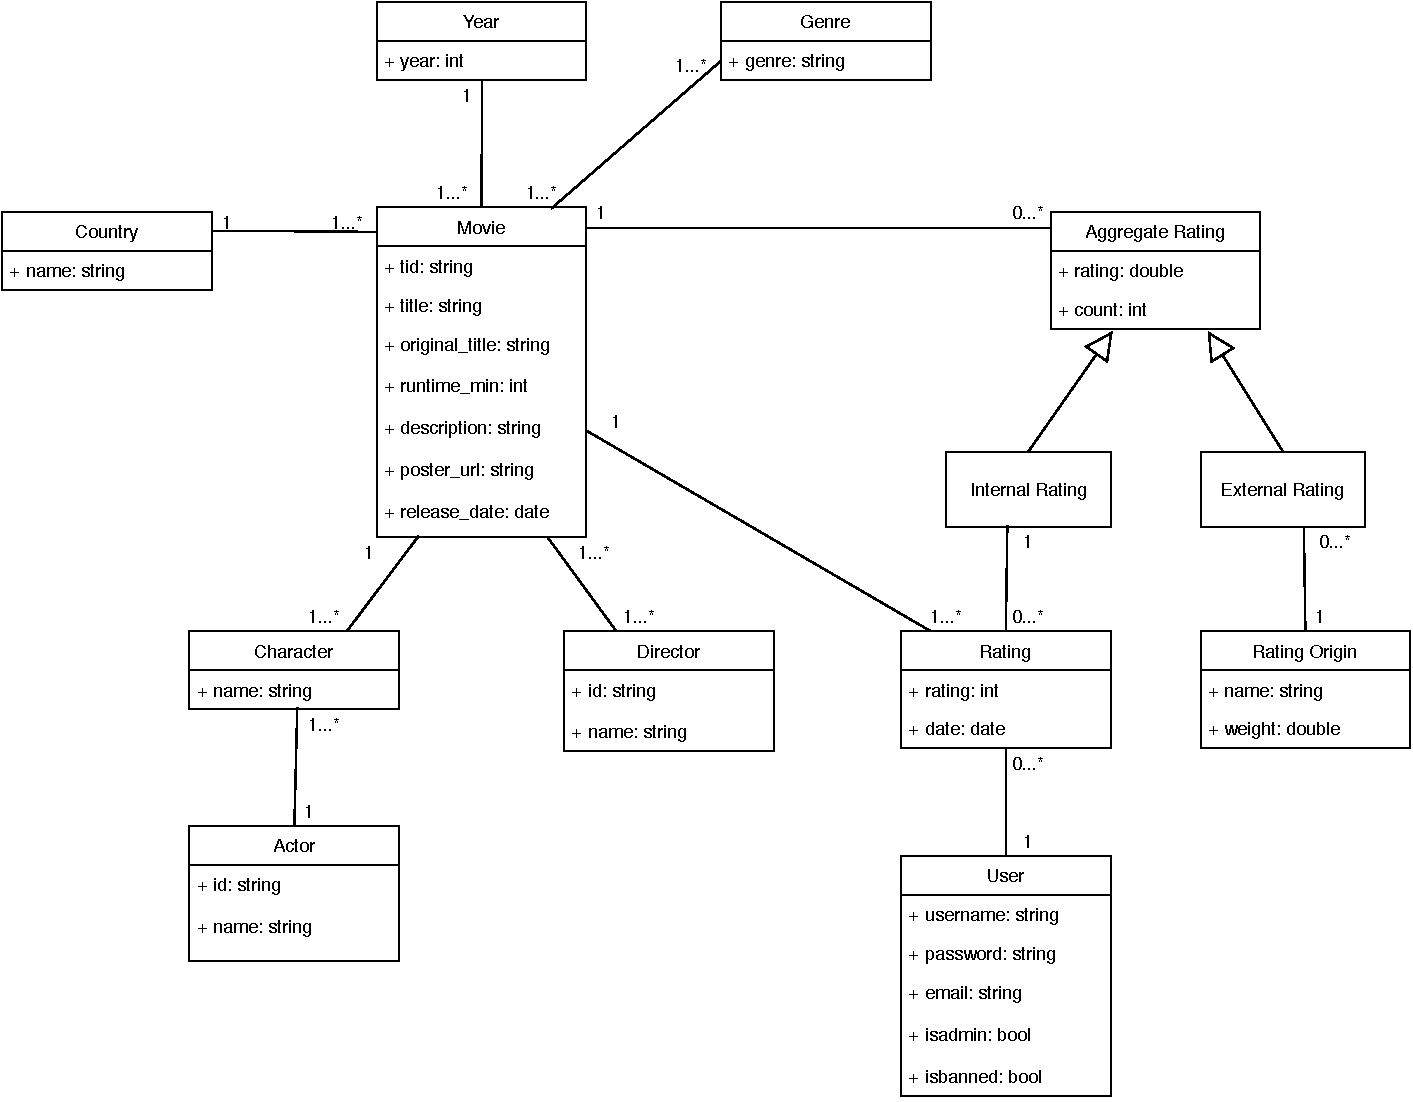
\includegraphics[width=\textwidth]{figs/class_diagram.pdf}
    \caption{Class diagram for the identified entities}
    \label{fig:class_diagram}
\end{figure}

The class diagram is shown in \cref{fig:class_diagram}. It was decided to show \emph{Country}, \emph{Year} and \emph{Genre} as separate entities as they are some of the fields over which aggregate statistics are calculated.

% ------------------------------------------------------------------------------

\clearpage
\subsection{Data model}
The data model is split in 3 different collections:
\begin{itemize}
	\item Movies (\cref{sec:movies})
	\item Users (\cref{sec:users})
	\item Ratings (\cref{sec:ratings})
\end{itemize}
In each following subsection, an example document is shown for every collection.

\subsubsection{Movies}
\label{sec:movies}

\begin{lstlisting}[language=json]	
{
	"_id": "tt7286456",
	"title": "Joker",
	"original_title": "Joker",
	"runtime": 122,
	"countries": ["USA", "Canada"],
	"original_language": "English",
	"year": 2019,
	"date": "2019-10-04",
	"description": "In Gotham City, mentally troubled comedian [...]",
	"storyline": "Joker centers around an origin of the iconic arch [...]",
	"tagline": "Put on a happy face.",
	"poster": "https://m.media-amazon.com/images/M/[...].jpg",
	"mpaa": "Rated R for strong bloody violence, disturbing behavior, [...]",
	"budget": 55000000,
	"gross": 1074251311, 
	"characters": [
		{
			"name": "Joker",
			"actor_name": "Joaquin Phoenix",
			"actor_id": "nm0001618"
		},
		...
	],
	"directors": [
		{
			"id": "nm0680846",
			"name": "Todd Phillips",
		}
	],
	"genres": ["Crime", "Drama", "Thriller"],
	"ratings": [
		{
			"source": "internal",
			"sum": 450,
			"count": 100,
			"weight": 1,
			"last_update": "2019-11-28 12:34:56"
		},
		{
			"source": "IMDb",
			"avgrating": 8.6,
			"count": 628981,
			"weight": 0.5,
			"last_update": "2019-11-28 12:34:56"
		},
		...
	],
	"total_rating": 4.43,
	"last_scraped": "2019-11-28 12:34:56"
}
\end{lstlisting}

\paragraph{Notes}
Character and director nested documents contain redundant data (person's name) that is introduced to reduce the number of seeks necessary to return the movie details
to the user.

This collection is mainly read-heavy since most fields will be written only once.
The only fields subject to change are the ones related to ratings. For these reasons,
we can afford many indices to speed-up the aggregations.

\paragraph{Indices} 
Indices on the following fields will be set for this collection:
\begin{itemize}
	\item \texttt{title}: speed-up sorting by title
	\item \texttt{title}, \texttt{original\_title} (text\ index): movie lookup 
			by name
	\item \texttt{countries} (multi-key index): filter and aggregation by country
	\item \texttt{genres} (multi-key index): filter and aggregation by genre
	\item \texttt{year}: filter and aggregation by year
	\item \texttt{date}: sorting by release date
	\item \texttt{characters.actor\_id} (multi-key index): filter and aggregation by actor
	\item \texttt{directors.id} (multi-key index): filter and aggregation by director
	\item \texttt{total\_rating}: filter and sorting by rating
	\item \texttt{last\_scraped}: fast lookup for next-to-be-scraped movie (oldest movie).
\end{itemize}

Among this fields, \emph{total\_rating} is the only one that will be updated 
frequently (all other fields with index are updated with the periodic scraper 
whose period is of some days). However it is necessary to efficiently fulfill 
many queries.

\subsubsection{Ratings}
\label{sec:ratings}

\begin{lstlisting}[language=json]	
{
	"_id": {
		"user_id": <ObjectId>,
		"movie_id": "tt7286456"
	},
	"date": "2020-01-20",
	"rating": 5
}
\end{lstlisting}

\paragraph{Notes}
The raw ratings are kept separated from the movie they refer for three reasons:
\begin{enumerate}
	\item single ratings are never shown to the user, except when the user 
			looks his own ratings or when the admin looks all ratings	
	\item they may be accessed per-user, per-movie (for calculating 	
			statistics) and globally (by the administrator). The optimization for one use-case would influence the performance of another.
	\item new ratings are expected to be frequently added and, thus, the use of 
		a nested document inside the \emph{movies} collection would be 
		infeasible because it would grow indefinitely. 
\end{enumerate} 

However, this choice mandates the introduction of indices for efficiently 
obtaining ratings of a single user and for getting the most recent ratings (admin use-case).

\paragraph{Indices} 
\begin{itemize}
	\item \texttt{\_id.user\_id}: speed up user ratings browse.
	\item \texttt{date}: speed up browsing user and global ratings.
\end{itemize}

\subsubsection{Users}
\label{sec:users}

\begin{lstlisting}[language=json]	
{
	"_id": <ObjectId>,
	"username": "joker",
	"password": "<HASHED PASSWORD>",
	"email": "joker@dccomics.com",
	"isadmin": True (optional),
	"isbanned": False (optional),
	"sessions": [
		{
			"session_id": "<session_id>",
			"expiry": "2020-01-28"
		},
		...
	]
}
\end{lstlisting}
\paragraph{Notes}
\emph{Username}, \emph{email} and \emph{session\_id} must be unique across the whole collection.

\paragraph{Indices} 
\begin{itemize}
	\item \texttt{username} (text index): find user by username
	\item \texttt{username}: find user by exact username
	\item \texttt{email}: find user by email
	\item \texttt{sessions.session\_id} (multi-key index): find user by session id
\end{itemize}

\subsection{Software Architecture}

The application will be made of the following 4 components:
\begin{itemize}
	\item \textbf{MongoDB}: a MongoDB cluster will be deployed with
		replication.
	\item \textbf{React Front-end}: web-based UI.
	\item \textbf{Java Back-end}: using \emph{Spring}, the \emph{Java back-end} will provide REST APIs to the \emph{React front-end}.
	\item \textbf{Updater ``bot''}: two Python scripts are needed in order to nightly update the DB with the latest movies and ratings: 
	\begin{enumerate}
		\item the \textbf{IMDb parser} periodically parses the IMDb dataset to add the latest movies.
		\item the \textbf{scraper} continuously parses the rating sources to update the ratings.
	\end{enumerate}
	These scripts will executes asynchronously from the \emph{Java back-end}.
\end{itemize}

% ------------------------------------------------------------------------------

\section{Database}

\subsection{Creation of the database}
The database is created from scratch starting from the public IMDb dataset available at the link \href{https://www.imdb.com/interfaces/}{https://www.imdb.com/interfaces/}.

We developed a Python script, in order to obtain the data in the form described in the Data Model. However, some information where missing. So we integrated missing information scraping them from the external rating sources while we were scraping for ratings.

Movies are saved into Json files and then ``upserted'' in MongoDB database with another simple python script with the use of the \textbf{UpdateOne} module. Update requests are appended to an array and served through the \textbf{bulk\_write()} function.

By enabling the \emph{upsert} functionality, we can reuse the same script to 
update the movie collection since movies that are not in the DB will be
inserted and movies that are already present will be updated. Note that it is
rare that a movie information will change so most of the time the \emph{upsert}
will do nothing to the stored movies.

\subsection{Scraping bot}
The aim of this bot, developed in Python (3.7) language, is to solve the problem of lack of data, indeed Movienator app needs a lot of movie information and details to work sensibly, so the scraper works providing from two main Web sources, MyMovies and IMDb, all types of data required, according to the ETL ("Extract-Transform-Load") paradigm.

We can identify two main uses of the scraper, as follow:
\begin{enumerate}
    \item Find missing sensible informations for stored movies.
    \item Update movies with most recent data, this operation is carried out periodically on each movie.
\end{enumerate}

Below are listed all the attributes collected by the scraper for each movie:

\begin{itemize}
    \item movie title;
    \item movie genre;
    \item URL to movie poster;
    \item movie description;
    \item public release date;
    \item aggregate rate of external source;
    \item extra attributes (storyline, tag-line, production country, budget ..)
\end{itemize}

\subsubsection{Software design according to ETL model}
% --------------------
\paragraph{Data extraction}
The very first step is data extraction, made possible by sequential HTTP requests (performed by Requests module), followed by the utilization of Beautiful Soup, a Python library for pulling data out of HTML and XML files.
Data, among different http responses, are retrieved by a JSON-LD tag, contained within html body of every single movie page.
\lstinputlisting[language=Python]{figs/code/get_ld_json.py}

Web indexing is made agile through two separate techniques:

\begin{enumerate}
    \item Across IMDb pages, every movie page is uniquely identified by imdb\_id, exploiting a standard URL format, "\emph{https://www.imdb.com/title/ttxxxxxxx/}", where \emph{"xxxxxxx"} is the integer id to locate the source. Since our database was built from IMDb, our DB uses the IMDB id, therefore we can just fetch the correct page.
    \item Exploiting MyMovies Web API, it's possible to find movies URL starting from their titles; "\emph{https://www.mymovies.it/ricerca/ricerca.php?limit=true\&q=yyyyyyy}", this is the query format, where the real argument (passed by GET method) is actually just one, \emph{"q"} and \emph{"yyyyyyy"} represents movie title (in Italian).
\end{enumerate}
% --------------------
\subsubsection{Data transformation}
All the input data, retrieved from Web, are parsed into Python dictionaries, exploiting json library methods applied to de-serialized data content, which is obtained by the \emph{``soup''} in the previous phase.

\lstinputlisting[language=Python]{figs/code/load_movie.py}
% --------------------
In the listing above, we can look at the code that performs a first processing of data, retrieved by the dictionary resulting from the de-serialization of the json content. Missing features are converted in properties with \emph{None} as a value, the objective is to deal with standard format dictionaries, solving the problem of heterogeneous data sources.

\subsubsection{Data loading: updating the database}
New scraped data, both for features update and addition, once parsed, are stored on MongoDB server by means of PyMongo API for Mongo DBMS. BSON is the standard format used to store documents and make remote procedure calls in MongoDB, luckily python dictionaries are directly mapped to BSON type as object and vice versa, so serialization (writings to Mongo) and de-serialization (readings from Mongo) processes are easily managed.

In order to perform the update on the least recently scraped movies, a \emph{last\_scraped} attribute is added (and modified) every time an update operation is executed from the script. The code listing below shows how to process consecutive movies, getting them by \emph{self.\-get\-Movies\-By\-Last\-Scraped} method and proceeding on integrating scraped data.
The scraper first marks the movie as scraped by updating the \emph{last\_scraped} attribute and then checks whether another scraper is scraping the same movie by comparing the \emph{last\_scraped} attribute that the \emph{find\_one\_and\_update} method returned (original DB document) with the one that the scraper retrieved earlier from the DB.

After having build the update dictionary, the scraper builds the list of operations to perform to the movie. In particular, old ratings are pulled and replaced with new ratings, then the \emph{total\_rating} is computed and updated along with other information (e.g. \emph{synopsis}, \emph{poster}, ...). In order to interact with Mongo database we exploited several methods from PyMongo module, such as: \texttt{find()}, \texttt{find\_one\_and\_update()}, \texttt{updateOne()}, \texttt{bulk\_write()}
All these methods take dictionaries as argument, with the exception of \emph{bulk\_write}, that is used for efficiency's sake.

\lstinputlisting[language=Python]{figs/code/update_mongo_movies.py}

% ------------------------------------------------------------------------------

\section{Back-end Implementation}
The API specification can be found in the \texttt{docs/api.md} file. This section will go through the implementation of the main APIs. 

\subsection{Java classes overview}
\begin{figure}
	\vspace{-2cm}
	\hspace{-1cm}
	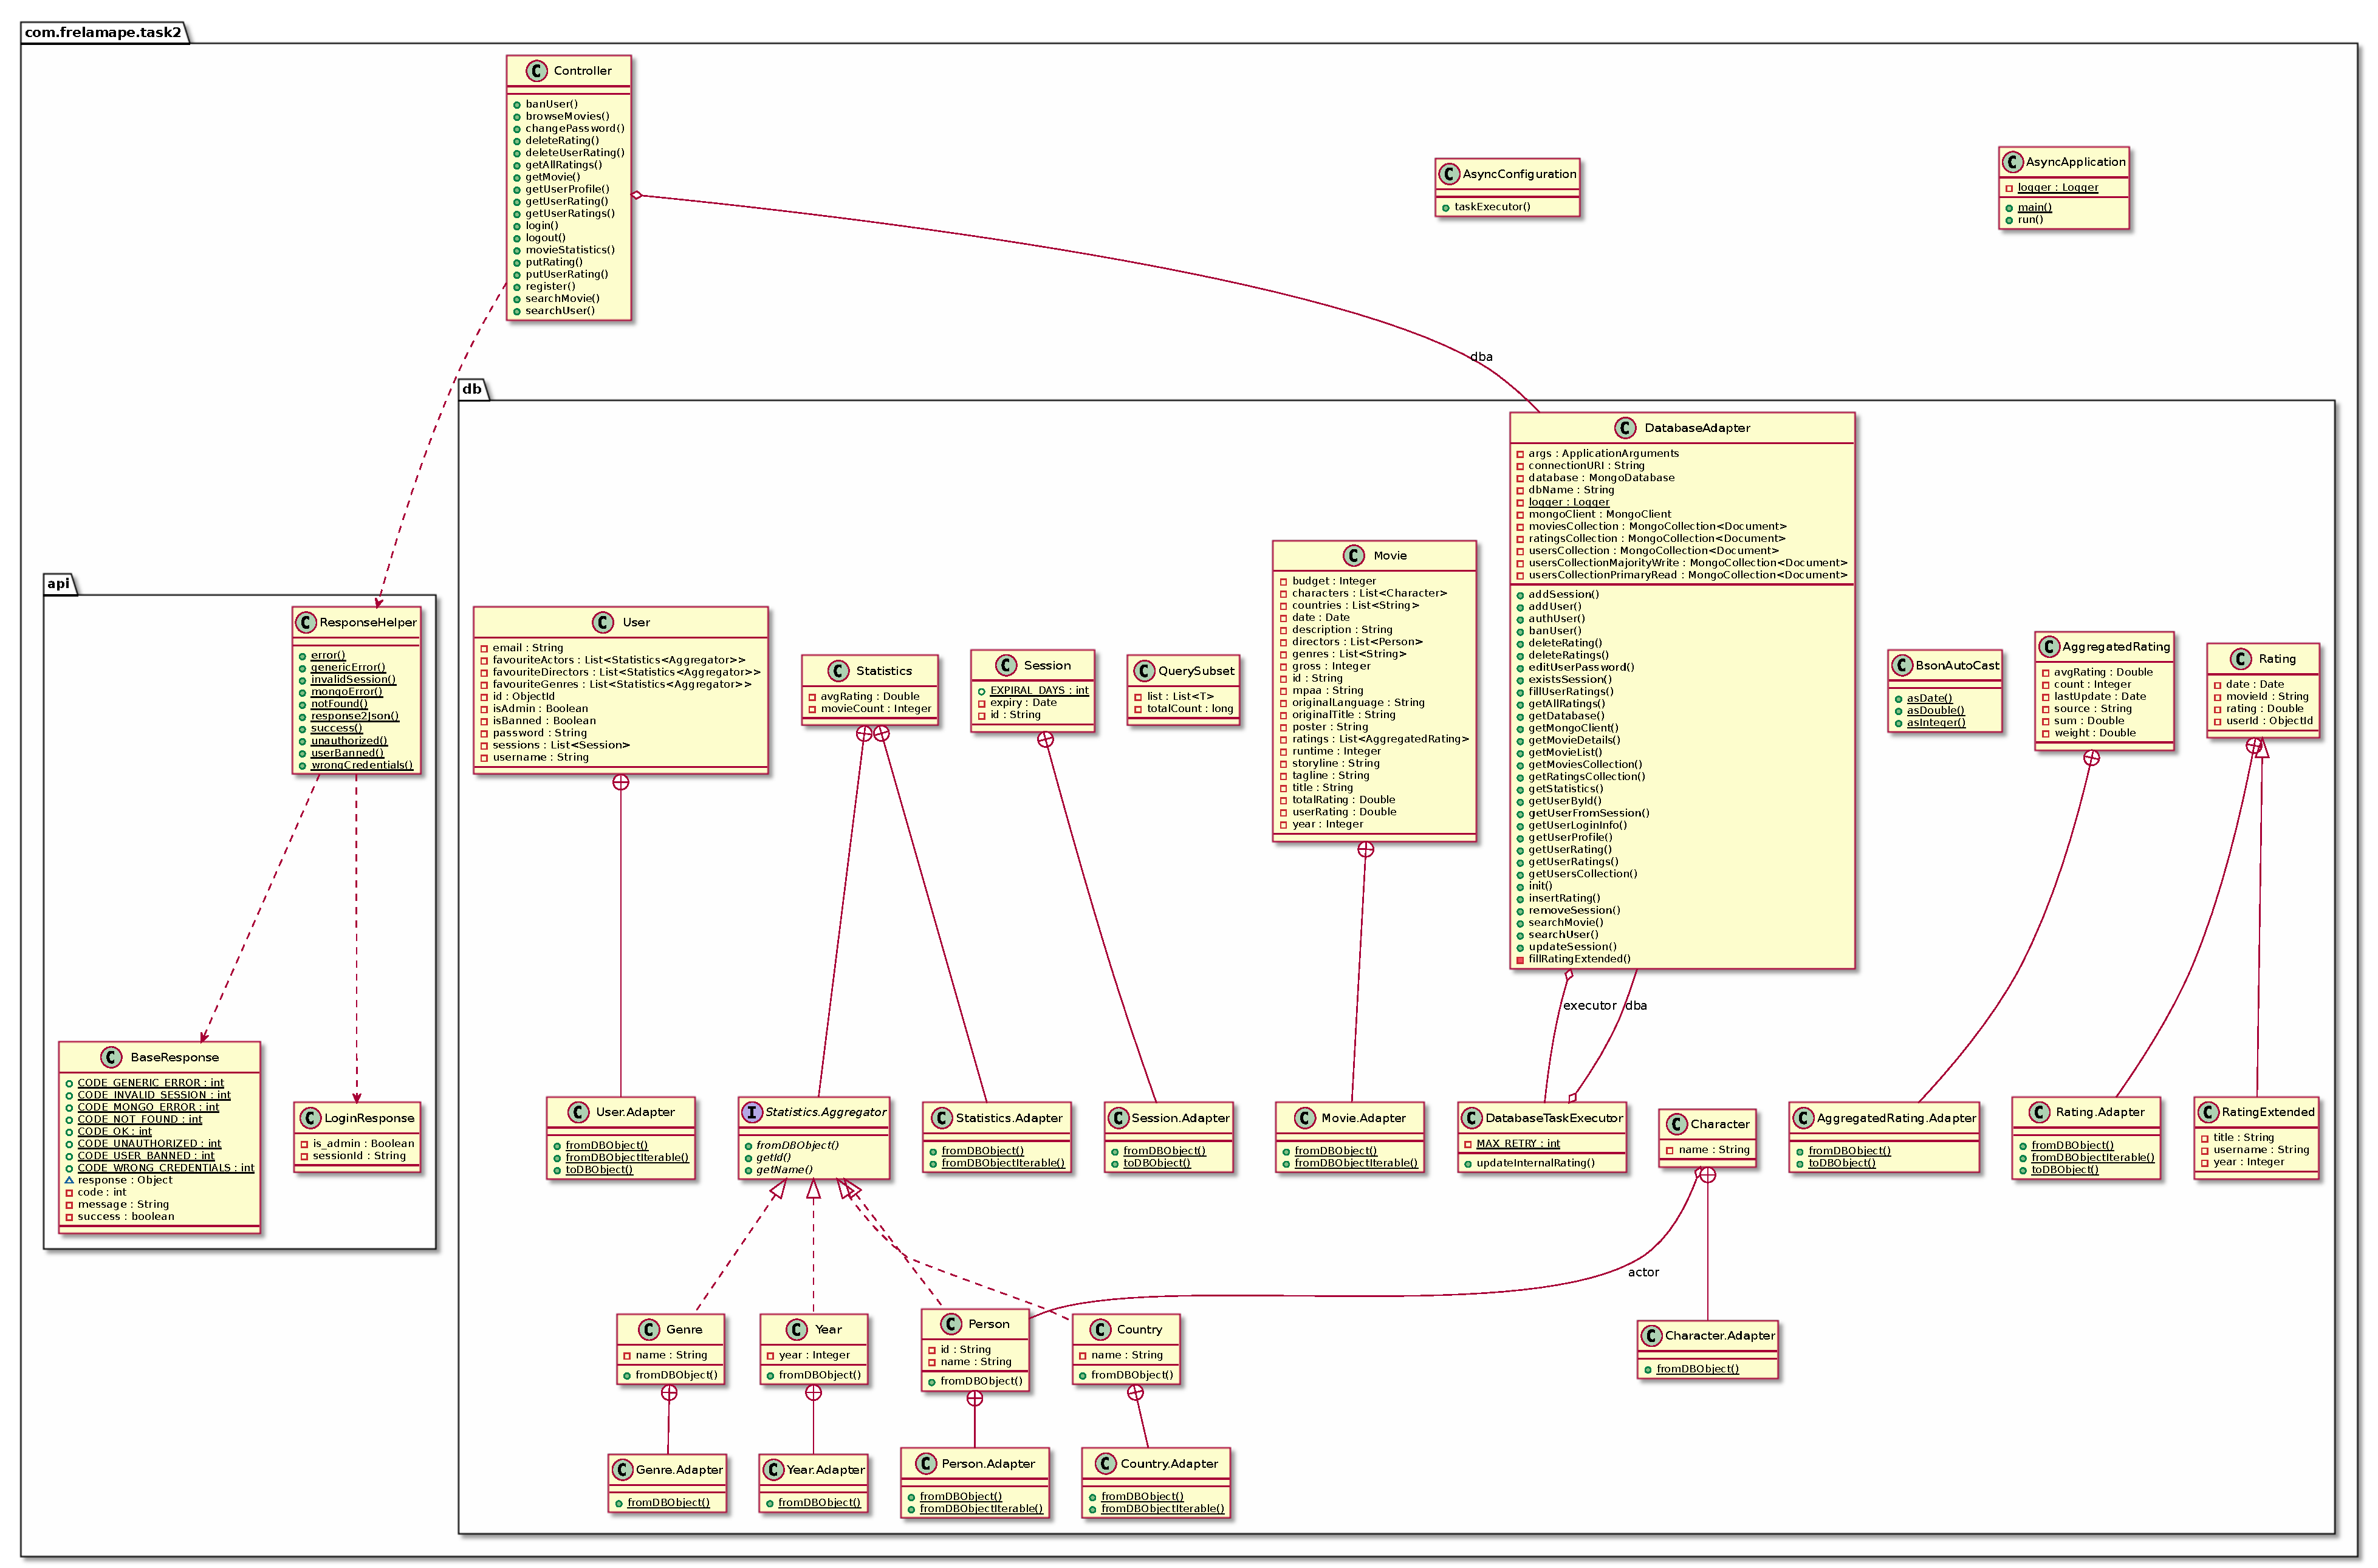
\includegraphics[height=18cm,angle=90]{figs/backend.pdf}
\end{figure}

In the previous page you can see the class diagram of the Java implementation.
The code is structured in 3 modules: 

\begin{itemize}
	\item the root module contains the Spring REST controller and other Spring-related classes;
	\item the \texttt{api} module contains the helper classes for formatting the output to the client as a JSON format
	\item the \texttt{db} module contains:
	\begin{itemize}
		\item the definition of the Java database objects (\emph{User}, \emph{Movie}, \emph{Rating}, ...). In addition, each object has an utility \emph{Adapter} nested class that provides static methods to easily convert a BSON document to the class instance.
		\item the \emph{DatabaseAdapter} class that contains the definition of all possible operation to the database.
		\item the \emph{DatabaseTaskExecutor} class that provides the definition of the asynchronous tasks that operate on the database (they are explained more in detail in the following sections).
		\item other utility classes (\emph{BsonAutoCast}, \emph{QuerySubset}, ...).
	\end{itemize}
\end{itemize}

\subsection{Authentication}
This subsection gives an overview over the most important APIs for authentication and session management. Passwords are stored in the database in the form of a Pbkdf2 hash (128-bit, 10k iterations) which is computed using the \emph{Spring Security} package.

\paragraph{Register}
In order to register a user, it must first be checked that no user with same username and password exists (snippet 1) and then, if no duplicate entry is found, the user can be added to the database (snippet 2). If creation was successful, a new session for the new user is then added (snippet 4). Any subsequent API call must be accompanied by the session identifier in order to identify the user (snippet 5).

\paragraph{Change Password}
This query (snippet 3) is simply done by matching the user by username and setting the new password hash.

\paragraph{Login}
In order to authenticate the user, the user document is retrieved from the database and then the password hash is checked with the password. 

\paragraph{Logout}
The session is removed from the DB (snippet 6).

\lstinputlisting[language=Java]{figs/code/authentication.java}

\subsection{Movies}
\subsubsection{Browse}
Returns a list of filtered movies with the given sorting. The result is paged.

\begin{enumerate}
	\item build a list of filters based on user specifications. People names are
			matched if all words in the query string are sub-strings of the full 
			name (this is done using a regex).
	\item Make the filter to pass to the \emph{find} function by ``and-ing'' all 
			conditions.
	\item Make the query:
		\begin{description}
			\item[find] all movies matching the conditions
			\item[sort] by the user-defined sort order
			\item[project] only movie important details
			\item[skip] the first \emph{n} pages
			\item[limit] the results to the page size
		\end{description}
\end{enumerate}

If user is logged in, a separate query will be done to fetch the user's ratings of the returned movies (\ref{sssec:userratings}).

\lstinputlisting[language=Java]{figs/code/browse_movies.java}

\subsubsection{Search}
During a search, movies that (fuzzy) match the entire query are returned sorted
by ``likelihood'' (meta text score, in MongoDB). Results are paged as before.

If user is logged in, a separate query will be done to fetch the user's ratings of the returned movies (refer to \ref{sssec:userratings}).

\lstinputlisting[language=Java]{figs/code/search_movie.java}

\subsubsection{Get Details}
Given a movie id, return all movie details. Code snippet not reported for brevity's sake.

\subsubsection{Browse Statistics}
This function is used to return aggregated statistics on movies based on one of the following information attributes:
\begin{itemize}
	\item genre
	\item year
	\item country
	\item director
	\item character
\end{itemize}
Before performing the aggregation, movies can be filtered as shown in the \textit{GetMovieList} API.
The statistics returned show the following informations about the aggregation attribute:
\begin{itemize}
	\item aggregated attribute
	\item average rating calculated on the aggregation
	\item number of movies present in the aggregation (calculated after filtering)
\end{itemize}
Results can also be sorted in ascending or descending order based on each of the previous attributes.

The aggregation pipeline is performed with the following code:

\lstinputlisting[language=Java]{figs/code/aggregation.java}

The \textbf{match} function uses the array of conditions "\textit{filters}" to perform all the filters in a single step. \textbf{Unwind} de-constructs the array field and returns a document for each array element (this is necessary for country, director and character fields). Then, the \textbf{group} function groups documents by the value expressed in the "\textit{realGroupBy}" and then applies accumulator expression to each group:
\begin{itemize}
	\item \textbf{Accumulators.first} sets "\textit{realGroupName}" as name of the group
	\item \textbf{Accumulators.avg} calculates the average rating of all the "\textit{total\_rating}" and saves them in the "\textit{avg\_rating}" attribute
	\item \textbf{Accumulators.sum} calculates the number of movies in the aggregation, by adding 1 to the variable "\textit{movie\_count}" for each movie
\end{itemize}
After that, the results are sorted with the \textbf{sort} function, where the argument "\textit{sorting}" is calculated as follow:

\lstinputlisting[language=Java]{figs/code/sorting.java}

Here, "\textit{realSortBy}" is the value to sort.

Finally, the \textbf{skip} and the \textbf{limit} functions are used to manage the display of the results.
%scrivere qualcosa sul ritorno?

\subsection{Ratings}
\subsubsection{CRUD operations}
A rating can be added, read, updated or deleted. Related code snippets are not shown for brevity's sake.

After a rating is updated, the corresponding movie rating information are asynchronously updated (refer to \ref{sssec:updateInternalRating}).

\subsubsection{Get all ratings for a user and list of movies}
\label{sssec:userratings}
This particular operation is done to add the user's ratings to a query result set. First the list of movie ids of the movies in the query result is built and then all ratings of the given user to any of those movies is returned.

By building the array of identifiers, just one query to the database is necessary.

\textbf{NB}: the number of movies will always be small due to paging (20).

\lstinputlisting[language=Java]{figs/code/fill_user_ratings.java}

\subsubsection{Browse All}
Administrators can browse all ratings in the collection in descending date order. Results are paged as seen in previous sections. Related code snippet is not shown for brevity's sake.

\subsubsection{Browse User Ratings}
Users can browse all their ratings in descending date order. Results are paged as seen in previous sections. Related code snippet is not shown for brevity's sake.

\subsubsection{Update Internal Rating}
\label{sssec:updateInternalRating}
After a rating is changed, the average internal rating and the total rating of the movie should be updated. This is done asynchronously after the update in order not to make the client wait for this additional operation.

The update takes in input the old and the new rating (one of them can be null in case of insertion or deletion) and consists in three parts:
\begin{enumerate}
	\item fetch the movie from the DB
	\item build the update request
	\begin{enumerate}
		\item Update \emph{internal rating}. The \emph{internal rating} nested document may be missing, in which case we need to push it. Otherwise, addition, deletion or modification must be correctly handled by incrementing \texttt{sum} and \texttt{count} appropriately.
		\item Update the \emph{total rating} by calculating the new average. If no rating is present any longer, the \emph{total rating} is unset.
	\end{enumerate}
\end{enumerate}

\textbf{NB: } the internal rating update is protected from concurrent modifications since it uses the atomic update operation \texttt{\$inc} to update the sum and the count. Furthermore, note also that all other aggregate ratings do not have the sum attribute but directly the average attribute since they are scraped. On the other hand, the update of the total rating is not consistent since another asynchronous entity (e.g. scraper) may overwrite it with stale information. However, this is not a big issue since at maximum just a few ratings will be lost among a big pool (thousands and more) so the average does not change much.

\lstinputlisting[language=Java]{figs/code/update_internal_rating.java}

\subsection{Users}
\subsubsection{Get Profile}
The user profile is composed by his personal information and his rating
statistics. The first part is just a \emph{find} operation. The second part uses an aggregation pipeline similar to the one used to find movie statistics with the difference that in the end results are sorted by descending rating and only first 3 results are shown to the user.

Note that this aggregation pipeline is, in a real scenario, very fast since a user will not have more than a few hundreds of ratings and ratings are indexed also by \texttt{user\_id} (so the match stage is extremely fast).

\lstinputlisting[language=Java]{figs/code/get_user_profile.java}

\subsubsection{Ban}
When a user is banned, a flag is set on its document and all his ratings are removed from the database (triggering the internal rating update). Code snippet is not reported for brevity's sake.

\subsubsection{Search}
User search works alike the movie search, taking advantage of a \emph{text index}, sorting results by best match and paging the result. Code snippet is not reported for brevity's sake.

\section{Authentication and replication}
\subsection{Configuration of the replica set}
Replication has been achieved through the set up of a MongoDB replica set in a remote cluster of 3 virtual machines provided by the University of Pisa.

A configuration document has been written, specifying the id of the replica set and the addresses of the machines. Additionally, a location tag was included. This could be useful if, in the future, the application is deployed to multiple data-centers for a more fine-grained control over the database requests (e.g. writes could be applied to at least one machine in every data-center before returning ). 

\begin{lstlisting}[language=json]	
rsconf = {
	_id: "replicaset0",
	members: [
	{_id: 0, host: "172.16.1.251:27017", tags: { location: 'unipi'} },
	{_id: 0, host: "172.16.1.162:27017", tags: { location: 'unipi'} },
	{_id: 0, host: "172.16.1.195:27017", tags: { location: 'unipi'} }
	]
}
\end{lstlisting}

By default MongoDB binds only to localhost, to allow connection through the network the \lstinline{mongod} daemon was started with the \lstinline{--bind_ip} flag.

\begin{lstlisting}[language=bash]
mongod 	--replSet replicaset0
		--dbpath ~/data/rs_db
		--oplogSize 200 
		--bind_ip 172.16.1.162
\end{lstlisting}
\subsection{Authentication}
In order to keep our system secure, authentication must be set-up.
A user responsible of handling our database, \textit{moviedb}, was created from the mongo shell.
\begin{lstlisting}
db.createUser(
	{
		user: 'lsmsdb',
		pwd: '******',
		roles: [ { role: "readWrite", db: "moviedb" } ]
	}
)
\end{lstlisting}

This is not enough since particular operations, like adding or removing new nodes to the replica set, require special privileges. The solution we choose was to create a superuser:

\begin{lstlisting}
db.createUser(
	{
		user: "lsmsdb_admin",
		pwd: "******",
		roles: [ {role: "root", db: 'admin' }],
		passwordDigestor : "server"
	}
)
\end{lstlisting}

The \lstinline{passwordDigestor} is an optional parameter which allows us to specify who has to digest the password (client or server). Since we use the SCRAM-SHA-256 mechanism, which is not compatible with the client, the server choice was forced.

After the users have been created, we run the MongoDB daemon with the authentication enabled, adding the \lstinline{--auth} flag:

\begin{lstlisting}[language=bash]
mongod 	--replSet replicaset0
		--dbpath ~/data/rs_db
		--oplogSize 200 
		--bind_ip 172.16.1.162
		--auth
\end{lstlisting}

All the connections from our Spring Boot server will now have to be authenticated with the \textit{lsmsdb} user we just created, while the administration of the cluster or of its node is to be done with \textit{lsmsdb\_admin}.

\subsection{Consistency, Availability and Partition tolerance}
The CAP theorem states that only two between consistency, availability and partition tolerance could be achieved in a database: our main service, providing movies infos and ratings, could work well even with outdated data.
Movie's description or title rarely change while average ratings should have a low variability: it is therefore the most convenient choice to increase our availability and partition tolerance.
This is not true for what concerns logins and accounts in general: e.g a password change should be set in stone or the user creation should grant login consistency. A bad user experience is the consequence of not handling correctly this aspects.

Different handling of the write and read requests depending on the data we want could be a reasonable solution.
The drivers connecting to the database can specify a \emph{WriteConcern} and a \emph{ReadPreference}: the first determines the number of members of the replica set that should have written the new data before a positive response is sent to the driver, the second option is about the possibility of reading from nodes other than the master.
The default configuration of MongoDB is a WriteConcern equal to 1 (only the primary server is updated) and a ReadPreference of 'primary' (we can read only from the primary). This means that, in case of a network partition excluding a number of nodes less than the majority and including the master, thus with the election of a new primary, consistency is not guaranteed since a write could have been made just before the partitioning (and the read would work just fine from the newly elected master).

What has been chosen, as already anticipated, is a differentiated approach depending on the request. To access the \lstinline{users} collection, the driver establishes three different connections with the database.

\begin{lstlisting}[language=Java]
mongoClient = MongoClients.create(connectionURI);
database = mongoClient.getDatabase(dbName);

moviesCollection = database.getCollection("movies").withReadPreference(ReadPreference.nearest());

usersCollection = database.getCollection("users").withReadPreference(ReadPreference.nearest());

usersCollectionMajorityWrite = database.getCollection("users").withWriteConcern(WriteConcern.MAJORITY);

usersCollectionPrimaryRead = database.getCollection("users").withReadPreference(ReadPreference.primary());

ratingsCollection = database.getCollection("ratings").withReadPreference(ReadPreference.nearest());
\end{lstlisting}

\lstinline{usersCollection} will be used for all the requests where we want high availability, like showing up the profile page or finding the user from the admin control page.

\lstinline{usersCollectionMajorityWrite} handles all the requests for which we want the updates to be permanent (e.g. password changes, new session id etc.): a write concern of 'majority' (which is computed against the total nodes in the replica set) protects us against network partition since no matter what happens to the nodes, as long as a majority is reached, the election system will make sure the successive primary node will have our write. Since the secondary nodes could or could not have it, when we want consistency we have to read only from the primary. Therefore, the \lstinline{usersCollectionPrimaryRead} will set the correct ReadPreference and will be used accordingly.

For what concerns the other requests, consistency is not strictly necessary and we would like our system to be highly available. For this reason, we keep the default write concern (equal to 1) and set the read preference to 'nearest', thus allowing reads from secondary nodes (which could have outdated informations).

\subsection{Test and evaluation}
\subsubsection{Election}
A test of the election mechanism has been done and, as we can see from the log reported below, it worked flawlessly: since no primary was seen for 10 seconds, a new election started (or, to be precise, a dry run followed by a \textit{real} run).
\lstinputlisting[language={}]{figs/code/election.log}

The candidate node was \lstinline{172.16.1.251} and received a positive vote from \lstinline{172.16.1.195}, while \lstinline{172.16.1.162} was unreachable (since it was down). A majority (2 out of 3) was reached and the secondary node transitioned to primary. It then caught up with the latest optime (row 19), cleaned the oplog and killed all the current user operations (row 25).

From the time of the dry run for election (19:55:36 and 242ms), which is 10 seconds after the last heartbeat in our case, to the new primary being up and running (19:55:36 and 269ms) only 27ms were elapsed: this is possible since the three nodes are connected to the same LAN, but certifies how the election mechanism is fast and efficient.

\subsubsection{Performance}
Another test we made is the evaluation of the performance, in terms of throughput (requests that can be served per second on peak load), of the database. We chose to test only the read performance of the most common API calls since these will be by far the most common. In particular, we individuated six kinds of API calls:
\begin{itemize}
	\item ``Simple browse'': movie browse without filters (10 movies per request).
	\item ``Filtered browse'': movie browse with filters (10 movies per request)
	\item ``Search'': movie search (10 movies per request)
	\item ``Details'': movie details
	\item ``Simple Statistics'': movie statistics without filters (10 groups per request)
	\item ``Filtered Statistics'': movie statistics with filters (10 groups per request)
\end{itemize}

For each type of API call, we generated a random subset of requests from which the testing application will randomly choose a request. 
The tests have been repeated three times, with a different number of servers in the replica set (1, 2 or 3).
We used \emph{siege} as a testing application, with 100 concurrent users and no delay between requests (benchmark mode), which executed for a minute for each run. Both back-end server serving the APIs and the \emph{siege} application ran on a server that was part of the replica set (this is the only member of the replica set that was always on during the experiments). All replica members are hosted on one of the virtual machines provided by the University of Pisa, each having 2 virtual CPU cores and a variable amount of RAM (from 2GB to 8GB, in the one hosting the Java back-end). The database contains around 50k movies. 

\begin{figure}[]
	\centering
	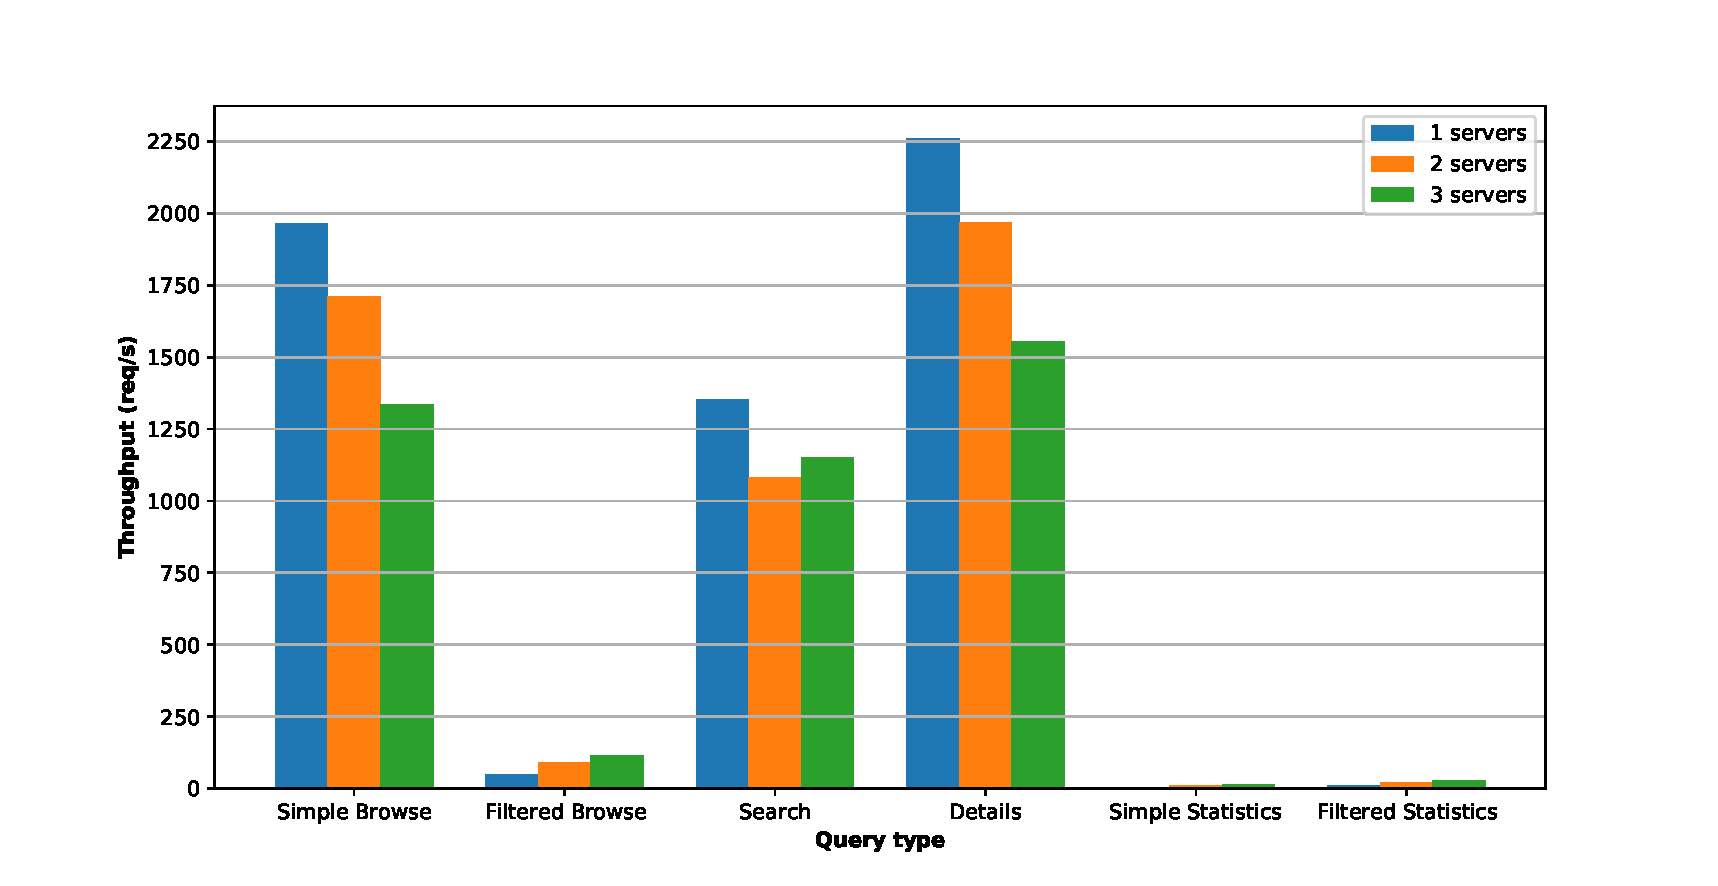
\includegraphics[width=\textwidth]{figs/siege_barplot_all.pdf}
	\caption{Results of the performance test for all 6 request types and for }
	\label{fig:barplot_all}
\end{figure}
\begin{figure}[]
	\centering
	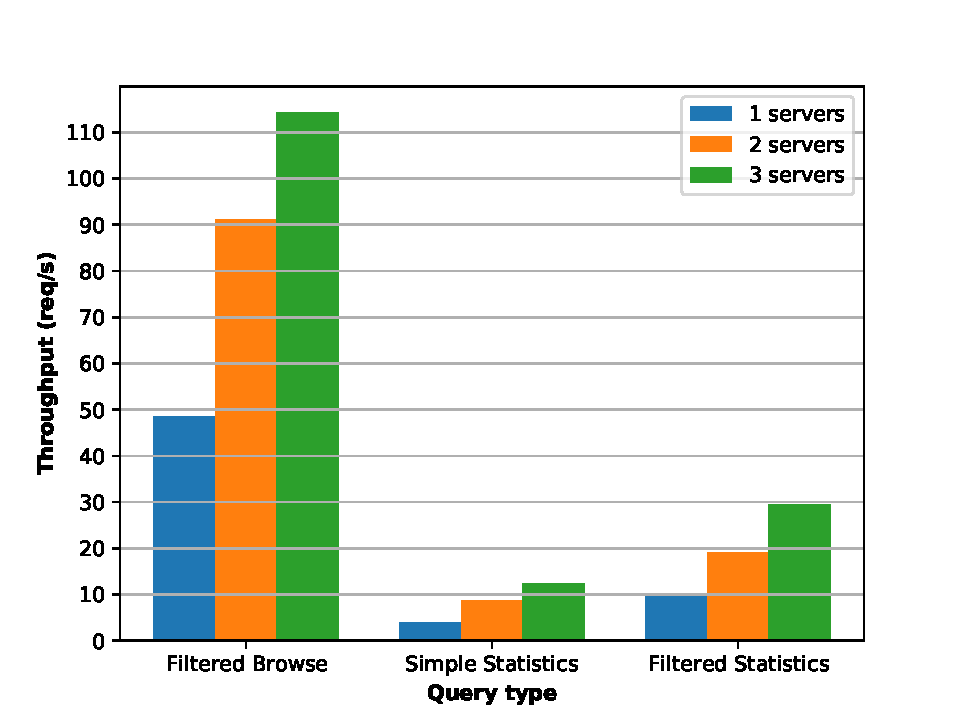
\includegraphics[width=\textwidth]{figs/siege_barplot_slow.pdf}
	\caption{Same plot as figure \ref{fig:barplot_all} but zoomed in to show slowest API calls.}
	\label{fig:barplot_slow}
\end{figure}

\paragraph{Results}
From figures \ref{fig:barplot_all} and \ref{fig:barplot_slow} we can note three things:
\begin{enumerate}
	\item ``Simple Browse'', ``Search'' and ``Details'' are much faster than the other queries. This was expected since these queries require little to 
	no effort to the database. 
	\item For the fast queries listed above, the performance actually lowers with an increased number of servers in the replica set. This is a consequence of the set-up we ran experiments on. The Java back-end server ran on the same node as the MongoDB node that was kept alive. Since these queries are IO-bound (in contrast, the other slower ones are computationally bound), when the Mongo driver, configured with the \emph{nearest} read preference, notices that the node is slow, it tries to balance read requests among the other nodes but, since they are remote, this actually introduces overheads.
	\item Statistics are faster on a filtered query then on a simple one. This is somehow counter-intuitive but keep in mind that the filter phase is very fast since it operates on indices and it reduces the number of elements to aggregate by possibly a large amount. Since the reduce phase needs to run on fewer records, its execution time is reduced.
\end{enumerate}

\paragraph{Possible solutions}
Since statistics are a core part of the Movienator website, a way to make them run faster must be found. The solution could be caching the most common statistics pages using an in-memory-database (e.g. Redis or Memcached). For instance, we could save the first few pages (e.g. 3 pages of 10 elements) for each possible aggregation (4) and visualization order (3). This would require space for just 360 records but would provide a huge impact on the server throughput. With regards to the problem of the fast queries being slow on a bigger cluster, a possible solution could be deploying a Java back-end server in each MongoDB node and set-up a load-balancer (e.g. HAProxy) to balance HTTP requests among the different back-ends. By doing so, latencies are minimized by locating the application near to the data source.

\subsubsection{Availability}
Some tests have been performed to test the ability of our MongoDB cluster to resist the failure of some nodes. Therefore some randomly chosen nodes have 
been shut down but the application kept responding to requests as expected. 

A more interesting test is the observation of the performance degradation (in terms of average response time) over time when nodes are removed from the replica set (fig. \ref{fig:crash_test}). In the following experiment, we ran 100 concurrent users making random back-to-back requests on the whole public section of Movienator. Every minute, a secondary node is either removed from the replica set or re-added, following the following sequence of alive node count: 3, 2, 1, 2, 3. 

\begin{figure}[]
	\centering
	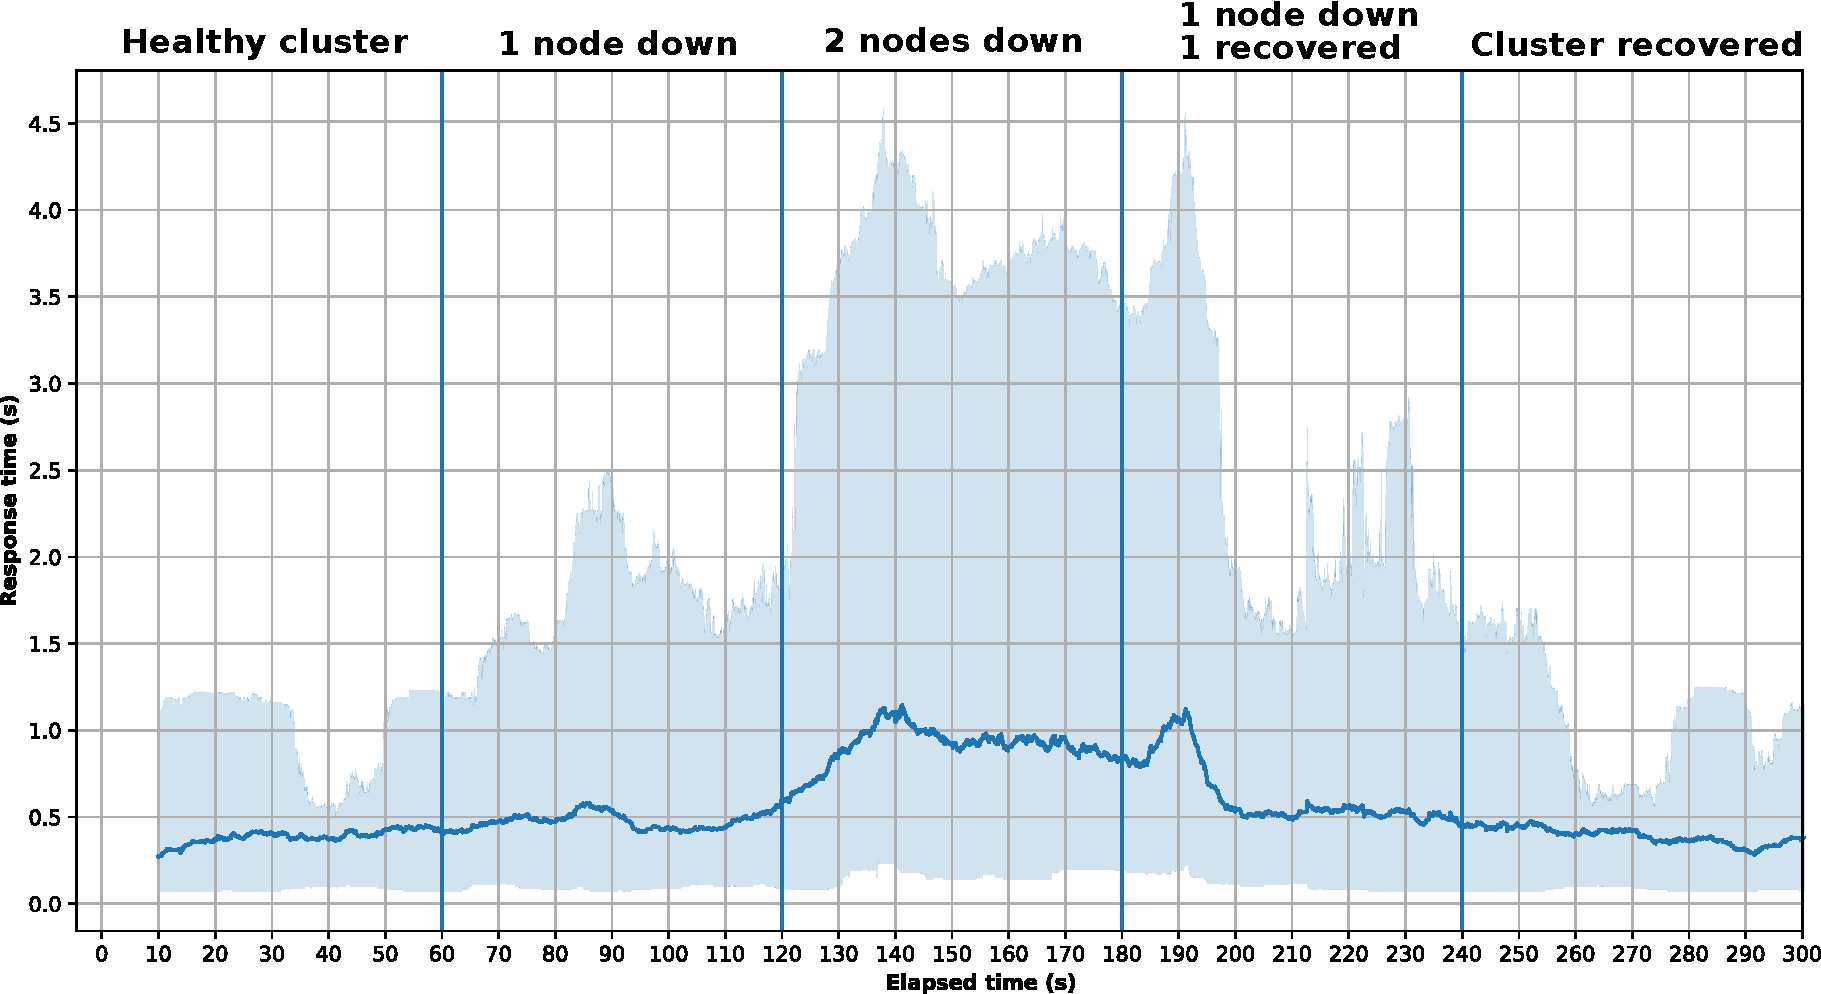
\includegraphics[width=\textwidth]{figs/crash_test.pdf}
	\caption{Plot of the moving average of the response time over time (line) and the 95-percentile to 5-percentile gap (area) inside the window. The window size of the moving average is 10s, therefore changes to the replica set are seen with a 10s delay. At t={60,120,180,240} the number of nodes in the replica set changes (3, 2, 1, 2, 3).}
	\label{fig:crash_test}
\end{figure}

\paragraph{Results}
From the figure we can make two observations:
\begin{enumerate}
	\item there is no substantial difference in the average response time with 3 and 2 nodes in the replica set. In contrast, the 95-percentile increases noticeably. This is explained by the fact that, as seen in the previous section, it's long running queries that are hurt harder by the missing server.
	\item when a node is restored, going from 1 to 2 nodes in the cluster, the users experience a transient spike of the response time before stabilising. A similar effect is not experienced when a node is removed from the set or when going from 2 to 3 nodes. This can be explained by the fact that when a node is bring up, it has to communicate with the primary to recover its state. This increased burden on the primary temporarily slows down requests. This does not happen when removing the nodes since, in this experiment, only secondary nodes have been removed.
\end{enumerate}

\subsection{Sharding}
Let's now discuss the possible introduction of sharding in our MongoDB. The discussion will be differentiated by collection.

\paragraph{Movies}
While the size of the \emph{movies} collection is quite large, it has a very low variability and it is not expected to grow fast over time. Furthermore, its contents easily fit into the memory of a single server. For these reasons, the sharding of the movie collection is not suggested.

\paragraph{Users}
Also the \emph{users} collection is not very large but, differently to the \emph{movies} collection, it grows faster and is composed of many small documents. If the number of users is small (up to 100000 order of magnitude), there is no need to shard them but, if this number grows to millions or even more, the collection could be sharded without problems since operations on users are a really small portion of all operations in Movienator and the additional overhead will not be a problem. The partitioning could be performed on the hash of the \emph{\_id} if the shards are co-located in the same geographical location or could be based on the TLD of the user's email in case of a geographically distributed database.

\paragraph{Ratings}
The \emph{ratings} collection is the fastest growing collection in the database. It is also possibly the biggest one and the only write-heavy one. Furthermore, users only access their own ratings, with the exception of admins. This makes it possible to flawlessly introduce sharding based on the \emph{user\_id} of the user. By doing so, all ratings of a user will be co-located on the same node. The administrators may experience a higher latency for getting the most recent ratings but it's not important.
Of course, there should be a significant amount of ratings to justify the introduction of sharding.

\end{document}